% LaTeX file for Chapter 03







\chapter{Results} \label{ch:Results}

%%%%%%%%%%%%%%%%%%%%%%%%%%%%%%%%%%%%%%%%%%%%%%%%%%%%%%%%%%%%%%%%%%%%%%%%%%%%%%%%
%%%%%%%%%%%%%%%%%%%%%%%%%%%%%%%%%%%%%%%%%%%%%%%%%%%%%%%%%%%%%%%%%%%%%%%%%%%%%%%%
%%%%%%%%%%%%%%%%%%%%%%%%%%%%%%%%%%%%%%%%%%%%%%%%%%%%%%%%%%%%%%%%%%%%%%%%%%%%%%%%
%%%%%%%%%%%%%%%%%%%%%%%%%%%%%%%%%%%%%%%%%%%%%%%%%%%%%%%%%%%%%%%%%%%%%%%%%%%%%%%%
%%%%%%%%%%%%%%%%%%%%%%%%%%%%%%%%%%%%%%%%%%%%%%%%%%%%%%%%%%%%%%%%%%%%%%%%%%%%%%%%

\section{Small Study Effect and Excess of Significance Tests} \label{sec:publication.bias.tests}




The meta-analyses fulfilling the criteria from chapter \ref{ch:dataset}, section \ref{sec:Processing}, are analysed with small study effects tests and excess significance tests. We will apply the tests on the original effect size measures, i.e. risk ratios, Hedges $g$ or log hazard ratios. Different tests are applied depending on if the outcomes are of type binary or continuous or survival.\\
Thus, we apply multiple tests on the same data. The results can then be displayed separately to compare the different tests. A histogram of $p$-values will summarize the overall evidence against the null-hypothesis of no publication bias, as displayed in Figure \ref{fig:test}. \\
``Excess significance'' denotes the excess of significant $p$-values testing method from \citet{excess.significance}, see \ref{sec:excess.significance}. For continuous and survival outcomes, the names refer to: 

\begin{itemize}
\item Egger's test, the weighted linear regression test as described in section \ref{sec:Egger}
\item Thompson and Sharp's test, the weighted linear regression test adjusted for between-study heterogeneity, section \ref{sec:Thompson}
\item Begg and Mazumdar's test, the rank test described in section \ref{sec:Begg}
\end{itemize}

For binary outcomes, the names refer to:
\begin{itemize}
\item Harbord's test, the likelihood score based test (section \ref{sec:Harbord})
\item Peter's test, the weighted linear regression with inverse sample size as explanatory variable (study size proxy) described in section \ref{sec:Peter}
\item R\"ucker's test, the test based on the arcsine transformation of proportions, in combination with Thompson and Sharp's regression test (section \ref{sec:Rucker})
\item Schwarzer's test, the rank based test using the expected event counts computed with the hypergeometric distribution (section \ref{sec:Schwarzer})
\end{itemize}

\begin{figure}
\begin{knitrout}
\definecolor{shadecolor}{rgb}{0.98, 0.98, 0.98}\color{fgcolor}

{\centering 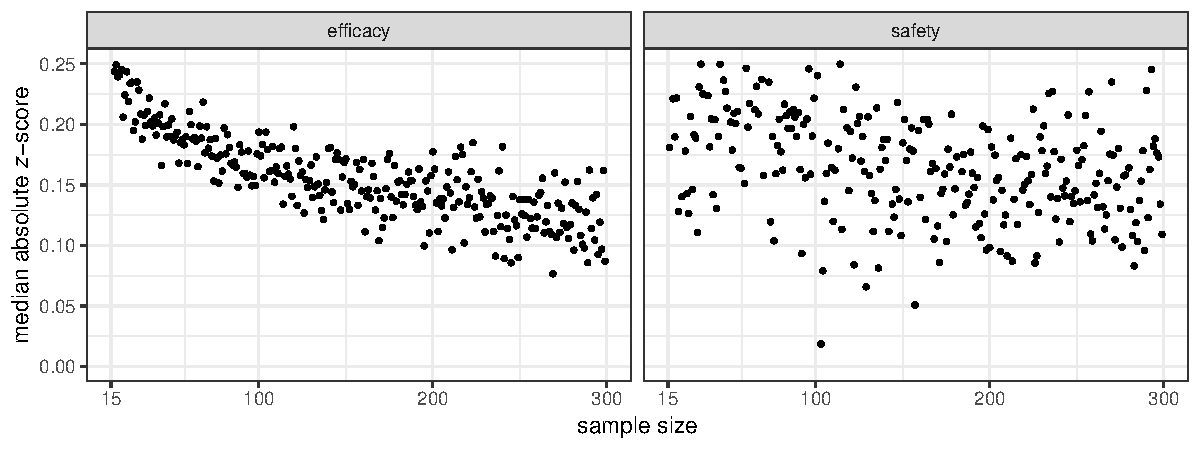
\includegraphics[width=\textwidth-3cm]{figure/ch03_figunnamed-chunk-2-1} 

}



\end{knitrout}
\caption{Histogram of the $p$-values for small study effect in meta-analyses. The testing method is indicated in the header, bin width is equal to 0.1. The significant proportion based on the threshold of 0.1 is displayed inside the figures.}
\label{fig:test}
\end{figure}

%Agreement table -> Chunck 1
The histograms in Figure \ref{fig:test} show that the distributions are (with the exception of Schwarzer's test) skewed to the right for all outcome types, indicating evidence for small study effects and excess significance, respectively. Moreover, the excess significance tests have a mode around $p = 0.4$. There is some discrepancy between continuous and binary data test results; the evidence for small study effects in continuous data is clearly larger. Survival outcome type results are quite different with very few evidence for small study effects, but almost 50\% of meta-analysis with significant excess significance tests. Note that the sample size of survival outcomes is small ($n$ = 39).\\
It cannot be seen in Figure \ref{fig:test} if the tests used are finding small study effects/excess significance for the same meta-analyses. A simple method to check the coincidence of test results is to compare scatterplots and empirical Spearman correlations between the test statistics. This is done in Figure \ref{fig:test.agreement}. Here, there is no separation between survival and continuous outcomes. The upper left rectangle is displaying binary outcome results and the lower right continuous and survival outcomes results.

\begin{figure}
\begin{knitrout}
\definecolor{shadecolor}{rgb}{0.98, 0.98, 0.98}\color{fgcolor}

{\centering 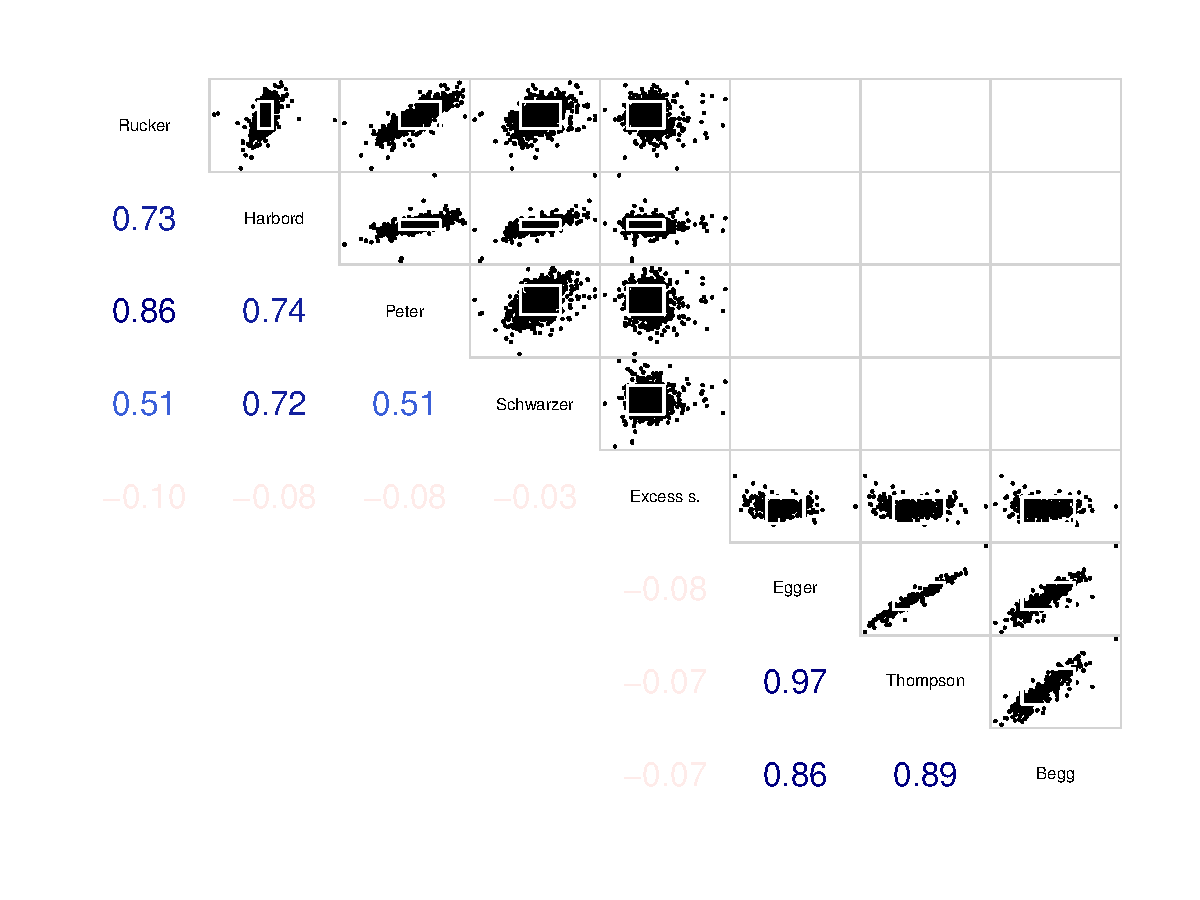
\includegraphics[width=\textwidth-3cm]{figure/ch03_figunnamed-chunk-3-1} 

}



\end{knitrout}
\caption{Pairs-plot for test statistics of small study effect and excess significance. The lower panel gives the Spearman correlations for the different test statistics, and the upper panel displays a scatterplot. The colors indicate magnitude and direction of the correlation coefficients. The rectangle with white borders displays the area within which both tests have absolute value < 1.64 (dots outside are statistically significant using the 0.1 threshold).}
\label{fig:test.agreement}
\end{figure}

The observed patterns on the scatterplots differ: Excess significance and small study effect test statistics do usually not align with each other, forming rather randomly scattered bulks of points. Regression based tests as Egger and Thompson which are methodically almost identical are closely aligned, which is reflected in large correlation coefficients. In general, small study effect tests align on the diagonal, but the extent to which they align differs. Continuous and survival outcome type tests align more closely than binary outcome tests. While correlation coefficients between binary outcome tests vary between each other, Harbord's test statistic has similar correlation coefficients with the other small study effect test statistics .\\
Because scatterplots and correlation coefficients can be misleading, also a Tukey mean-difference or Bland-Altman of transformed $p$-values plot is shown for four scenarios in Figure \ref{fig:mean.diff.test}:
\begin{itemize}
\item For Egger's and Thompson's tests, which is supposedly the most similar test and should show the least deviations and systematic errors
\item For Egger's and excess significance tests
\item For Harbord's and R\"ucker's tests
\item For Harbord's and excess significance tests
\end{itemize}

This can be justified since all tests are supposed to measure the evidence for publication bias. For the plots, the $p$-values of the tests are transformed on the entire continuous scale by a logit transformation $f(x)  = \log\frac{p}{1-p}$). The mean $p$-value (($f$($p$-value no. 1) + $f$($p$-value no. 2))/2) is then displayed against the difference between the $f$($p$-value). If no systematic errors and biases exist between the measurement methods, then 

\begin{itemize}
\item the mean of the differences should be around zero (systematic error) 
\item the points should scatter independently on the $y$-axis and no general increase or decrease with the mean of the transformed $p$-values should be visible
\end{itemize}

Although this is not formally tested, the last criterium seems not to be given when comparing small study effect and excess significance tests. With decreasing mean, the difference gets more negative, and vice versa, such that one would predict that the excess significance $p$-values are more ``extreme'' in both directions. -- In the appendix, it can be seen that this is reproducible with the remaining small study effect tests (not there yet) -- However, the systematic error between the compared tests is close to zero, and small study effect tests do probably not show bias when compared to each other. \\
The confidence intervals can be used as limits of agreement, which gives, after back-transformation, around 0.9 for Egger's and Thompson's test, and around 0.99 for Harbord's and R\"ucker's tests. This suggests that correspondence between the tests is not very good in general. 

\begin{figure}
\begin{knitrout}
\definecolor{shadecolor}{rgb}{0.98, 0.98, 0.98}\color{fgcolor}

{\centering 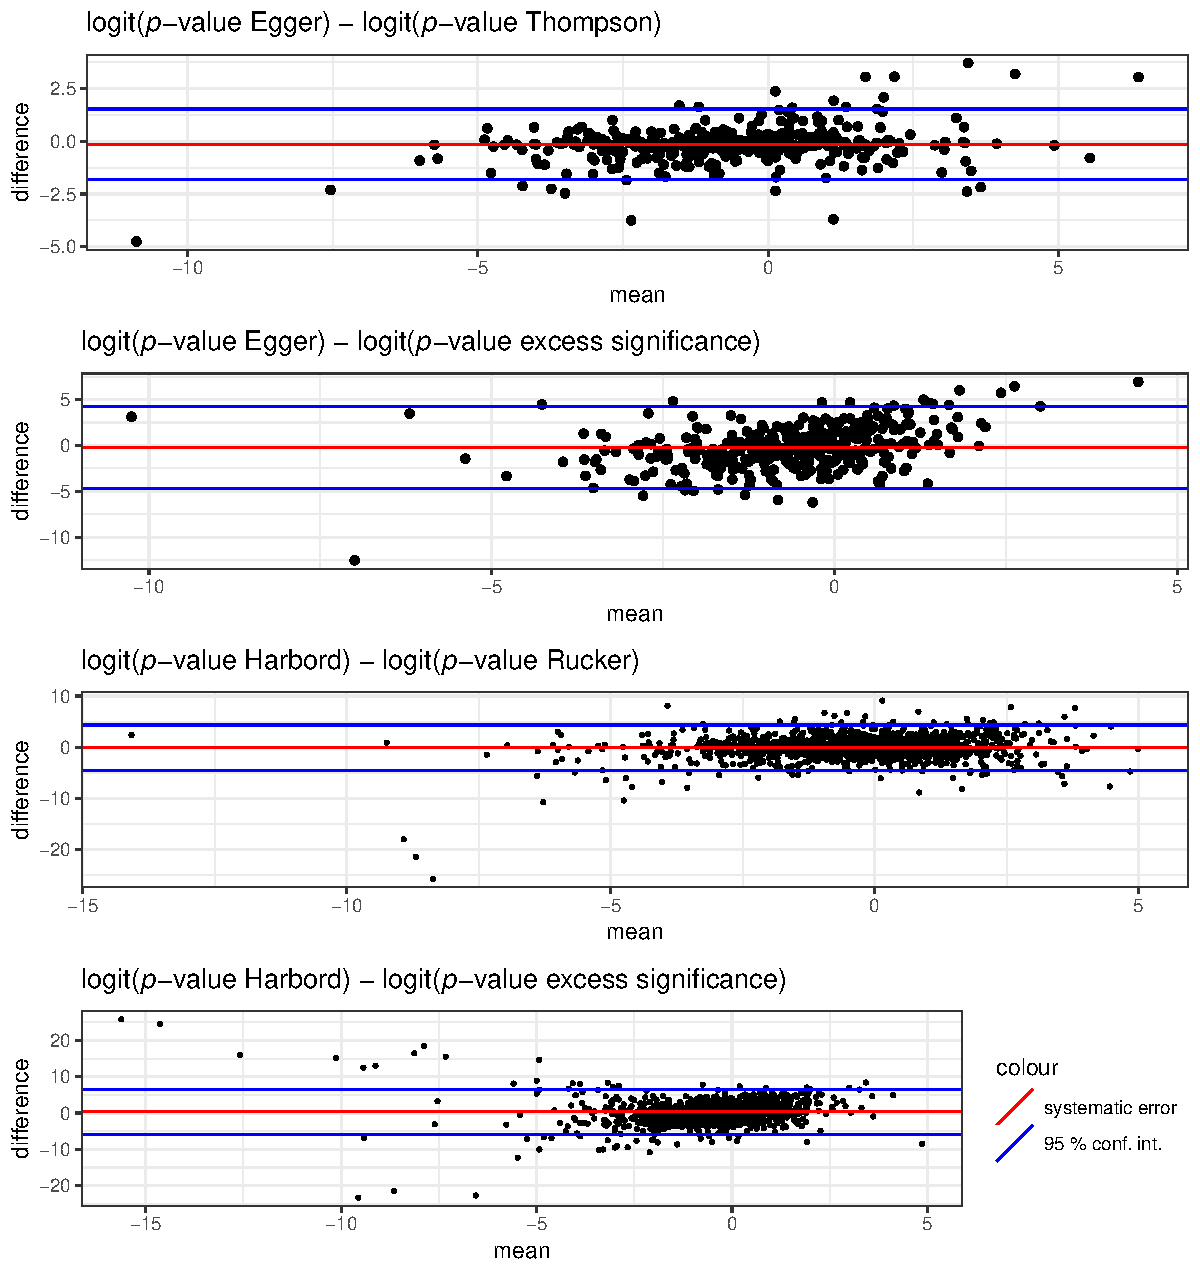
\includegraphics[width=\textwidth-3cm]{figure/ch03_figunnamed-chunk-4-1} 

}



\end{knitrout}
\caption{Mean - difference plots for logit transformed $p$-values. The mean of logit transformed $p$-values is displayed on the $x$-axis and the difference on the $y$-axis. Blue and red lines display the systematic error and the confidence intervals of the systematic error (limits of agreement).}
\label{fig:mean.diff.test}
\end{figure}

The previous results suggest that the results will also differ substantially after applying the common dichotomization of $p$-values. We expect that some proportion of the meta-analysis will only be significant for a certain test, and this is indeed observed in Table \ref{number.sig.tests}. It displays the percentage of meta-analyses with a certain number of significant test results.

% latex table generated in R 3.5.1 by xtable 1.8-3 package
% Mon Jul  1 14:05:10 2019
\begin{table}[ht]
\centering
\begingroup\footnotesize
\begin{tabular}{ccc}
  \hline
Count & Binary Outcomes & Continuous and Survival \\ 
  \hline
0 & 65.1 \% & 70.4 \% \\ 
  1 & 16.8 \% & 9 \% \\ 
  2 & 8.8 \% & 7.5 \% \\ 
  3 & 5.9 \% & 10.8 \% \\ 
  4 & 3.1 \% & 2.3 \% \\ 
  5 & 0.4 \% & - \\ 
   \hline
\end{tabular}
\endgroup
\caption{Counts Number of significant test results per meta-analysis, separated
       for outcome types. Last entry for continuous and survival outcomes is empty since one test less was 
       applied} 
\label{number.sig.tests}
\end{table}


Here, it is difficult to say if continuous and survival or binary outcome types show better agreement, since more tests are applied in the binary case, and the continuous and survival outcome type tests have in general more positive findings. Very few meta-analyses are significant, irrespective of the test used, but around 67\% of the dataset is not significant, no matter which test is used. \\
When only looking at small study effect tests, 29.1\% of binary outcome tests and 26.2\% of survival and continuous outcome tests had at least one significant result. This also suggests that the overlap between small study effect tests and excess significance is small. After applying the Bonferroni correction for multiple testing, this shrinks to 10.9\% for binary and 12.1\% for continuous and survival outcomes. \\
To compare significant findings for small study effect tests and excess significance tests, we limit ourselves to comparison with Harbord's or Egger's test. 23.5\% of binary outcome analyses had at least one of the two test $p$-values being significant, and equivalently, 25.4\% for continuous and survival outcomes. The numbers change to 14\% for binary outcomes and 14.4\% for continuous and survival outcomes after applying the Bonferroni correction. \\
3.2\% have significant Harbord's test result and significant excess significance test result  (1.1\% with Bonferroni). Of the continuous outcomes, we have 5.7\% with Egger's test and 1.8\% with Bonferroni correction. 

%%%%%%%%%%%%%%%%%%%%%%%%%%%%%%%%%%%%%%%%%%%%%%%%%%%%%%%%%%%%%%%%%%%%%%%%%%%%%%%%
%%%%%%%%%%%%%%%%%%%%%%%%%%%%%%%%%%%%%%%%%%%%%%%%%%%%%%%%%%%%%%%%%%%%%%%%%%%%%%%%
%%%%%%%%%%%%%%%%%%%%%%%%%%%%%%%%%%%%%%%%%%%%%%%%%%%%%%%%%%%%%%%%%%%%%%%%%%%%%%%%
%%%%%%%%%%%%%%%%%%%%%%%%%%%%%%%%%%%%%%%%%%%%%%%%%%%%%%%%%%%%%%%%%%%%%%%%%%%%%%%%
%%%%%%%%%%%%%%%%%%%%%%%%%%%%%%%%%%%%%%%%%%%%%%%%%%%%%%%%%%%%%%%%%%%%%%%%%%%%%%%%

\section{Small Study Effects Adjustment}


\subsection{Change in Effect Size after Adjustment} \label{sec:change.size}

Since there's evidence for publication bias when applying small study effect and excess significance tests, we apply small study effect adjustment methods to correct for small study effect tests. \\
We will see that consequences of adjustment can be; 
\begin{itemize}
\item first, the absolute size of the treatment effect can be smaller than the classical meta-analysis treatment effect, which is expected if publication bias
is the cause for the small study effect.
\item secondly, the effect can be larger than before in meta-analysis. In this case, the small study effect must be not due to publication bias for large effects (``true'' publication bias), but due to bias for small effects (``negative publication bias'').
\end{itemize}

In section \ref{sec:comparison.tests.adjustment}, it will be followed up on the latter point. For now, we will examine the extent and the frequencies of the two scenarios. \\
To compare the effects of adjustment between meta-analyses, the outcome measures are transformed to Hedges $g$ (standardized mean differences) and Fisher's $z$-score (see section \ref{sec:transformation.effectsizes} for details). The effect of adjustment can additionally be compared to either random or fixed effects meta-analysis. \\
Figure \ref{fig:adjustment.size} displays the difference $\delta$ between the observed meta-analysis pooled treatment effect and the adjusted treatment effect, $\hat{\theta}_M - \hat{\theta}_\textrm{Adj.}$. The absolute value $|\hat{\theta}_M|$ is taken and the sign of $\hat{\theta}_\textrm{Adj.}$ is adjusted accordingly such that all effects are mirrored to one side. $\delta > 0$ is equivalent to $\hat{\theta}_\textrm{Adj} < \hat{\theta}_M$, a reduction of the original effect size. For better illustration, some very large and very small differences have been omitted in the $z$-score and Hedges $g$ histograms; they are shown in Table \ref{missing.differences}. Table \ref{adjustment.difference} shows the quantiles and means for the various differences and additional information.\\

\begin{figure}
\begin{knitrout}
\definecolor{shadecolor}{rgb}{0.98, 0.98, 0.98}\color{fgcolor}

{\centering 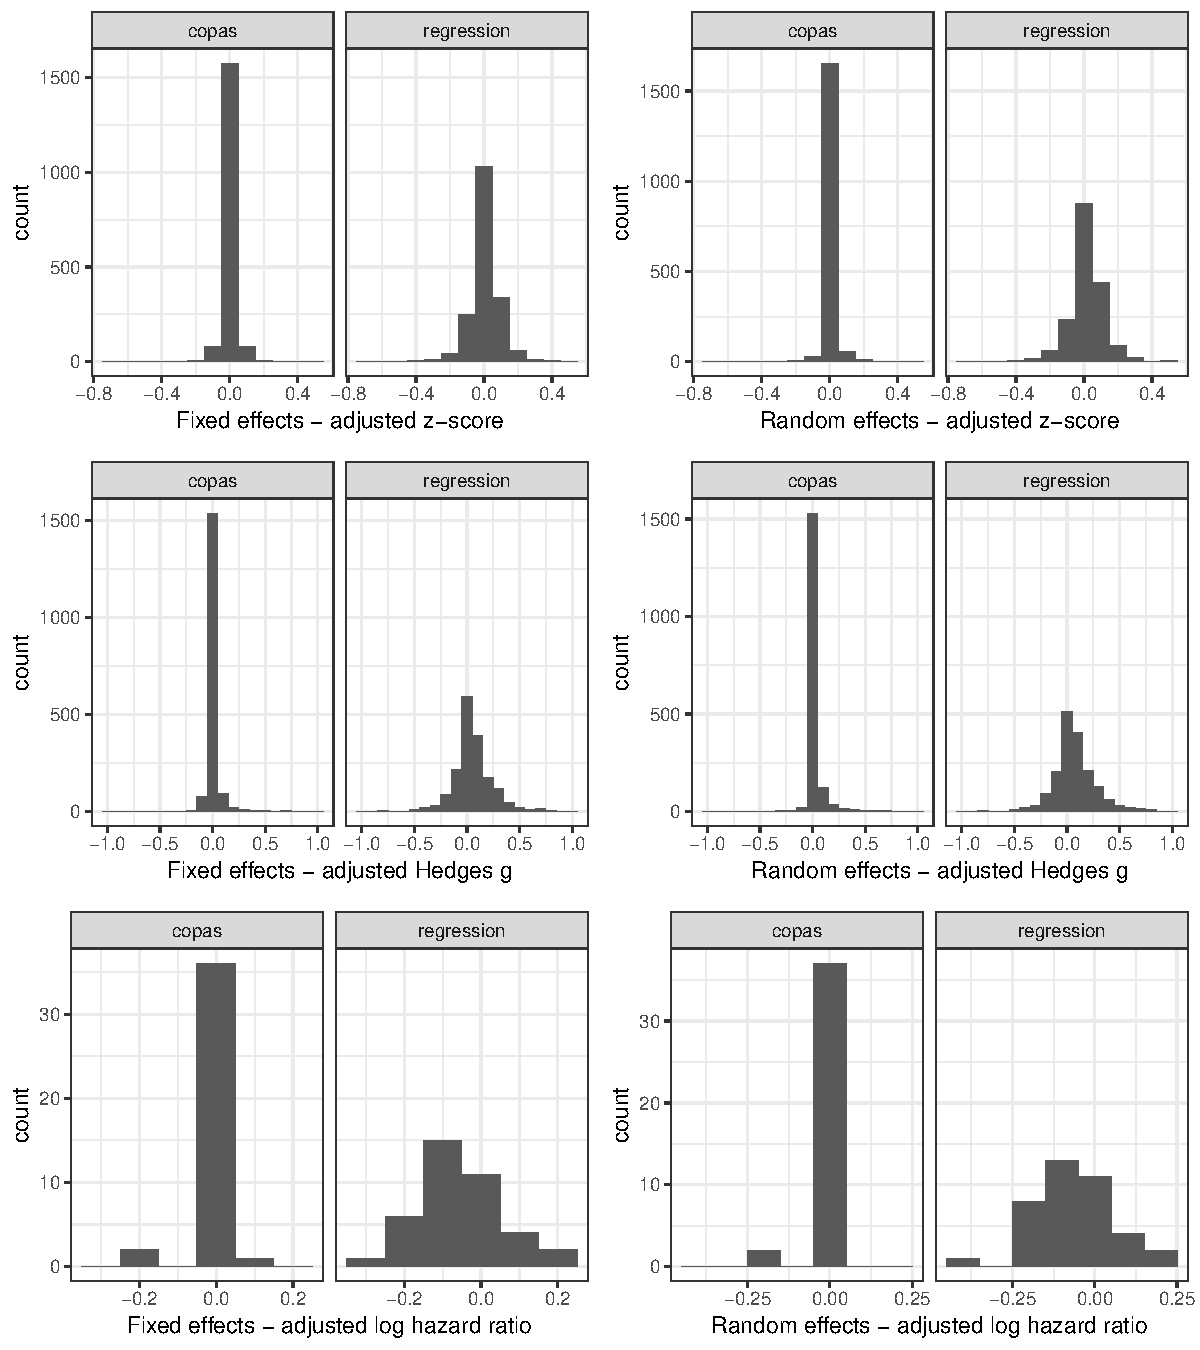
\includegraphics[width=\textwidth-3cm]{figure/ch03_figunnamed-chunk-7-1} 

}



\end{knitrout}
\caption{Histogram of the treatment effect differences between meta-analysis and adjusted meta-analysis. Negative differences indicate greater adjusted effect sizes than meta-analysis effect sizes. The bins are centered at zero.}
\label{fig:adjustment.size}
\end{figure}

% latex table generated in R 3.5.1 by xtable 1.8-3 package
% Mon Jul  1 14:05:13 2019
\begin{table}[ht]
\centering
\begingroup\scriptsize
\begin{tabular}{lcccccccccr}
  \hline
 & 5\% & 25\% & 50\% & 75\% & 95\% & mean & = 0 (\%) & $>$= 0 (\%) & $>$ 0 (\%) & No adj. est. (\%) \\ 
  \hline
z: Fixed - Copas & -0.05 & -0.01 & -0.00 & 0.01 & 0.05 & -271.73 & 4.76 & 48.67 & 43.91 & 71.54 \\ 
  z: Random - Copas & -0.00 & 0.00 & 0.00 & 0.00 & 0.04 & -263.62 & 71.65 & 89.42 & 17.77 & 71.54 \\ 
  z: Fixed - Regression & -0.13 & -0.03 & 0.01 & 0.05 & 0.14 & 0.01 & 0.00 & 52.44 & 52.44 & 0.17 \\ 
  z: Random - Regression & -0.15 & -0.03 & 0.02 & 0.07 & 0.18 & 0.02 & 0.00 & 57.64 & 57.64 & 0.17 \\ 
  g: Fixed - Copas & -0.05 & -0.01 & 0.00 & 0.01 & 0.09 & 0.02 & 22.76 & 59.14 & 36.38 & 60.96 \\ 
  g: Random - Copas & -0.00 & 0.00 & 0.00 & 0.00 & 0.14 & 0.03 & 63.29 & 87.49 & 24.20 & 60.96 \\ 
  g: Fixed - Regression & -0.23 & -0.04 & 0.03 & 0.13 & 0.38 & 0.05 & 0.00 & 61.96 & 61.96 & 0.00 \\ 
  g: Random - Regression & -0.24 & -0.03 & 0.05 & 0.16 & 0.42 & 0.06 & 0.00 & 64.06 & 64.06 & 0.00 \\ 
  Log h.r.: Fixed - Copas & -0.03 & 0.00 & 0.00 & 0.00 & 0.02 & -0.01 & 41.03 & 38.46 & 79.49 & 61.54 \\ 
  Log h.r.: Random - Copas & -0.03 & 0.00 & 0.00 & 0.00 & 0.00 & -0.01 & 66.67 & 15.38 & 82.05 & 61.54 \\ 
  Log h.r.: Fixed - Regression & -0.21 & -0.14 & -0.07 & 0.01 & 0.15 & -0.06 & 0.00 & 33.33 & 33.33 & 0.00 \\ 
  Log h.r.: Random - Regression & -0.22 & -0.15 & -0.07 & 0.03 & 0.15 & -0.06 & 0.00 & 33.33 & 33.33 & 0.00 \\ 
   \hline
\end{tabular}
\endgroup
\caption{Quantiles and Means of the differences between meta-analysis pooled treatment effects and small study adjusted treatment effects. The column with the names ``> 0'' give the percentages of estimates larger than zero or larger or equal zero. The column ``No adj. est.'' gives the percentage of missing estimates due to non-significant publication bias test (for Copas) and computational errors. The row names indicate which outcome measure, meta-analysis method and adjustment method is used. Abbreviations are used for z-score (= z) and Hedges g (= g).} 
\label{adjustment.difference}
\end{table}




Adjustment leads most often to reduction of treatment effect estimates, as can be seen by the size of the bins of the right part of the histograms in Figure \ref{fig:adjustment.sue}. The difference between the bins on the right and left side of the zero-centered bin is however not very large in general. The seeming exception of the Copas selection model in the case with $z$-scores and fixed effects reference requires closer examination: Copas selection model substitutes its estimates with random effect estimates when it finds no evidence for small study effects. Thus, when comparing Copas with Fixed effects, we compare most often random effects with fixed effects estimates. The effect of adjustment by Copas can therefore only be seen when comparing random effects estimates with fixed effect estimates: we can see in Table \ref{adjustment.difference} that we have, for $z$-score, 18.4\% reduced effect sizes compared to 10.3\% (= 100\% - 89.69\%) increased effect sizes. Thus, the Copas selection model also has a larger proportion of reduced effect sizes compared to amplified.\\
%This resolves the case for the seeming exception and for Hedges $g$'s, 24.4\% and 12.46\% (Table \ref{adjustment.difference}. 
Also, there are more reduced effect sizes if random effects meta-analysis is used as a reference effect size. When Hedge's $g$ is used as an effect measure, there are (substantially) more reduced effect sizes. \\
The means in Table \ref{adjustment.difference} suggest that the average reduction is small (the means of Copas in the first two rows for $z$-score are caused by one very large value, see Table \ref{missing.differences}). To recall some other findings out of Table \ref{adjustment.difference}: 5\% or 90 cases have their $z$-score reduced by more than 0.15 by regression adjustment (and 5\% or 90 increased by -0.13, fixed effects reference). Also, Hedges $g$ is reduced by 0.39 compared to fixed effects estimates in 5\% or 90 meta-analyses (or increased by 0.24).



\subsection{Change in Evidence for Treatment Effects} \label{sec:change.evidence}
Adjustment for small study effects in meta-analysis will not only provide new effect sizes, but also standard errors thereof. Thus, also the evidence for efficacy of a treatment can be obtained, which is usually summarized in a suitable test statistic or $p$-value. It is of interest if and how the evidence for treatment effects changes if adjusted for publication bias.\\
The Wald test statistics $p$-value for fixed and random effects meta-analyses and Copas and regression adjusted treatment effects have been calculated. They are shown in Figure \ref{fig:adjustment.stat} for meta-analysis based on $z$-score, Hedges $g$ and log hazard ratios. \\
It can be seen that evidence for a treatment effect decreases after adjusting for publication bias. It does so more for Hedge's $g$ compared to $z$-scores, and for regression adjustment compared to Copas selection model. 
%Also, the evidence decreases for random effects meta-analyses compared to fixed effects meta-analyses. 
In the case of log-hazard ratio adjustment, the adjustment has only negligible impact on the $p$-values. \\
Also, Copas selection method has a very small impact on the evidence compared to random effects meta-analysis, at least using $z$-scores (again, we should rely on comparisons to random effects meta-analysis to evaluate Copas method). \\ 
% Interestingly, in contrast to the small study effect tests, there seems to be no large difference between adjusted continuous and binary meta-analysis test statistics --appendix--
%Figures \ref{fig:adjustment.stat.z} for the adjusted $z$-scores, \ref{fig:adjustment.stat.smd} for the adjusted Hedges $g$ and Cohen's d and \ref{fig:adjustment.stat.log.hazard.ratio} for the adjusted log hazard ratios.

\begin{figure}
\begin{knitrout}
\definecolor{shadecolor}{rgb}{0.98, 0.98, 0.98}\color{fgcolor}

{\centering 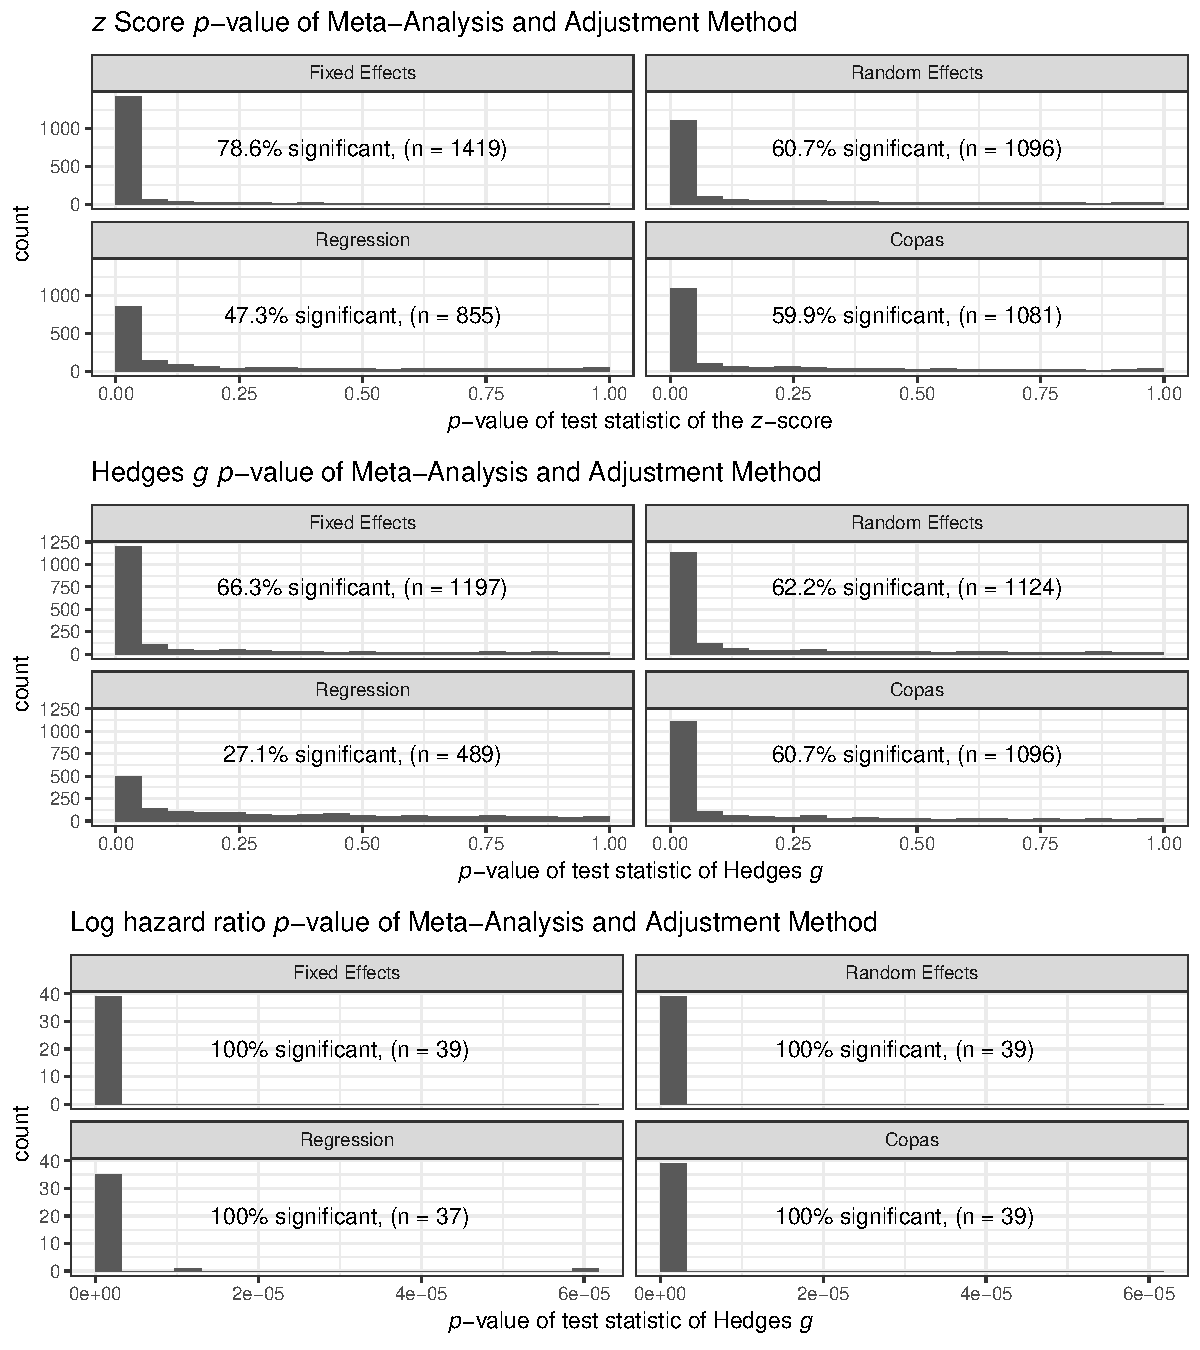
\includegraphics[width=\textwidth-3cm]{figure/ch03_figunnamed-chunk-9-1} 

}



\end{knitrout}
\caption{Histogram of the Wald test-statistic $p$-value of meta-analysis and adjusted pooled treatment effect, based on different treatment effect measures. The method is indicated in the header, bin width is set to 0.05. The significant proportion based on the threshold of 0.05 is displayed inside the figures.}
\label{fig:adjustment.stat}
\end{figure}

The Copas selection model also gives an estimate of the number of missing studies. It finds that 0 are missing, which corresponds to 0\% from all \ensuremath{2.8945\times 10^{4}} analysed studies. Figure \ref{fig:copas.missing} shows a histogram of the overall fraction of missing studies. Note that we have excluded 0 out of 1806, for which no Copas selection model estimate, but a random effects estimate was retained because the algorithm initially found no evidence for small study effects.

\begin{figure}
\begin{knitrout}
\definecolor{shadecolor}{rgb}{0.98, 0.98, 0.98}\color{fgcolor}

{\centering 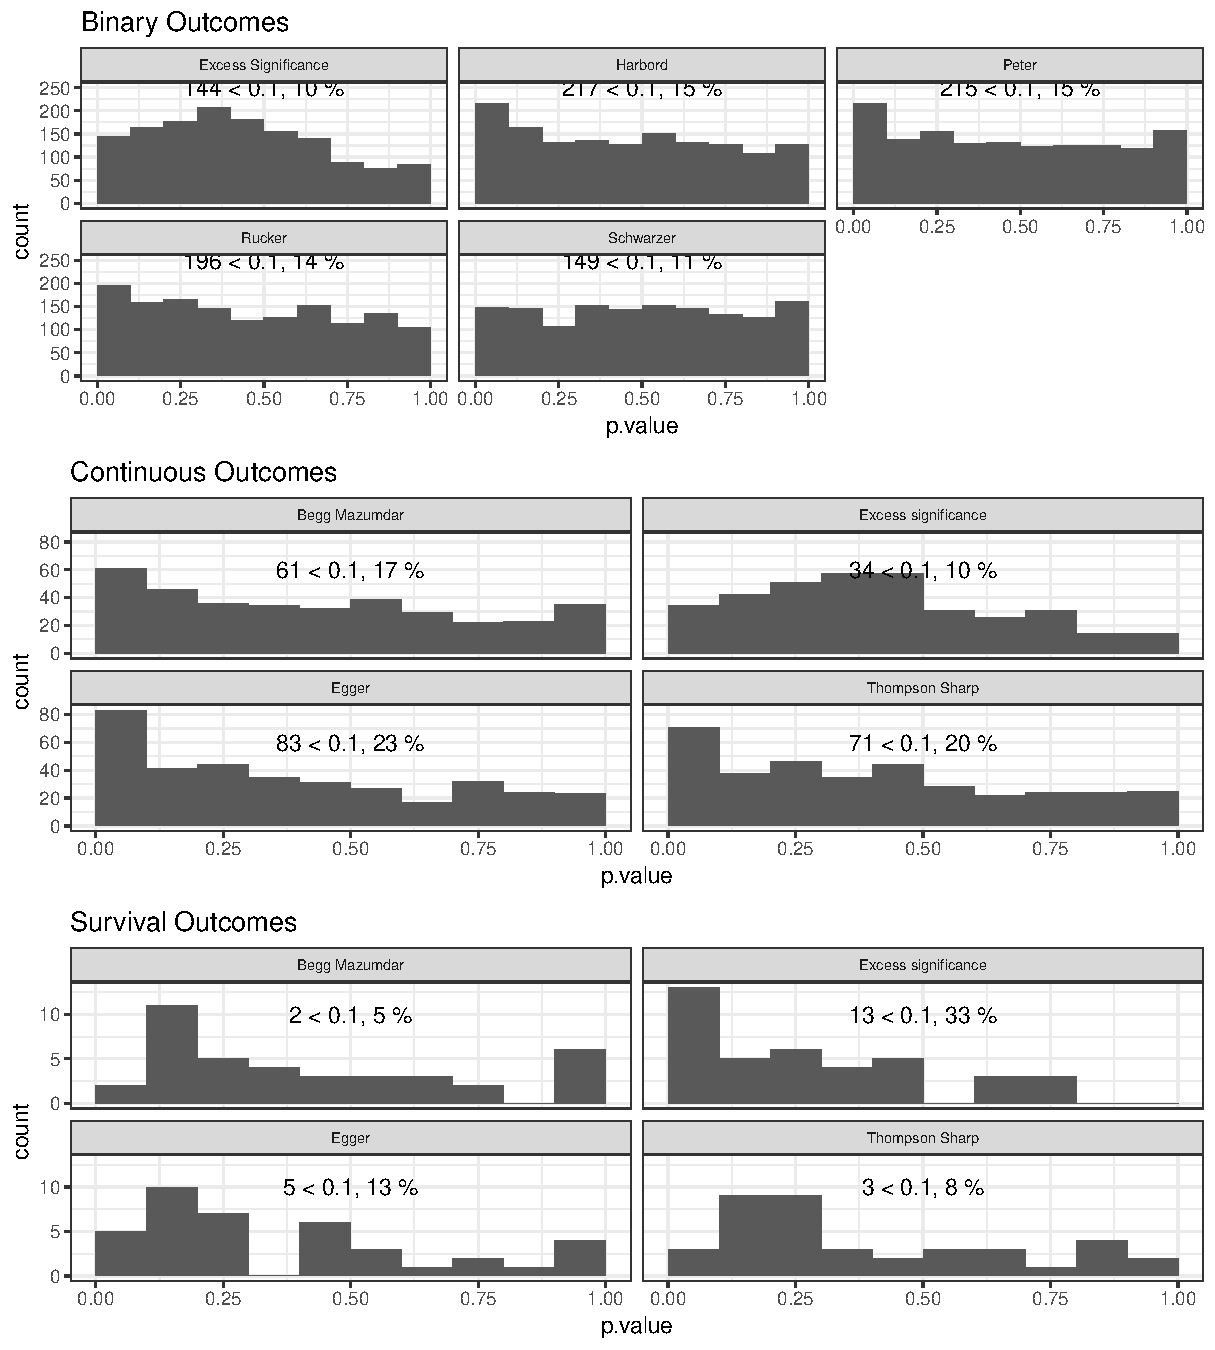
\includegraphics[width=\textwidth-3cm]{figure/ch03_figunnamed-chunk-10-1} 

}



\end{knitrout}
\caption{Histogram of the fraction of missing studies from the total number of studies in a meta-analyses (only data shown where Copas estimate was obtained, thus \\$n =$ 0)}
\label{fig:copas.missing}
\end{figure}

We can see that in some occasions, the method finds more than half of all studies are missing. In most occasions, the estimate of missing studies is zero, as can be seen in Table \ref{copas.missing}. The discrepancy between mean and median may indicate that the estimate of 0\% missing studies depends somewhat on these extreme cases. As can be written of from Table \ref{copas.missing}, 5\%, \ie 0 meta-analyses have 17.6 or more studies missing: in fact, these 5\% most extreme make up for 0, more than 30\% of missing studies.

% latex table generated in R 3.5.1 by xtable 1.8-3 package
% Mon Jul  1 14:05:15 2019
\begin{table}[ht]
\centering
\begingroup\footnotesize
\begin{tabular}{lrrrrrrr}
  \hline
 & = 0 & 5\% & 25\% & 50\% & 75\% & 95\% & mean \\ 
  \hline
Missing fraction & 321 & 0 & 0 & 0.1 & 0.3 & 0.9 & 0.2 \\ 
  Missing study number & 321 & 0 & 0 & 1.4 & 5.2 & 17.6 & 4.1 \\ 
   \hline
\end{tabular}
\endgroup
\caption{Fraction of missing studies and estimates of missing studies with their zero counts (``= 0''), quantiles and means.} 
\label{copas.missing}
\end{table}






% latex table generated in R 3.5.1 by xtable 1.8-3 package
% Mon Jul  1 14:05:15 2019
\begin{table}[ht]
\centering
\begingroup\tiny
\begin{tabular}{lcccrrrrrrrr}
  \hline
meta.id & file.nr & comparison.nr & subgroup.nr & z fixed & z random & z Copas & z regression & g fixed & g random & g Copas & g regression \\ 
  \hline
2009 & 2009 & 1 & 1 & 0.31 & 0.36 & 0.31 & 0.43 & 0.70 & 0.70 & 0.70 & 2.48 \\ 
  2068 & 2068 & 2 & 0 & 0.29 & 0.35 & 0.29 & 0.42 & 0.68 & 0.68 & 0.68 & 2.57 \\ 
  52528 & 52528 & 1 & 0 & -0.75 & -0.69 & -0.50 & -0.26 & -1.19 & -1.53 & 0.18 & -0.52 \\ 
  60546 & 60546 & 1 & 1 & 0.17 & 0.24 & 0.17 & 0.34 & 0.53 & 0.53 & 0.53 & 1.65 \\ 
  70389 & 70389 & 1 & 1 & -0.08 & -0.07 & 15.62 & -0.04 & -0.13 & -0.13 & -0.13 & -0.05 \\ 
  73769 & 73769 & 3 & 1 & -0.09 & 0.00 & 7148.96 & 0.02 & -0.01 & -0.12 & 0.01 & 0.04 \\ 
  79113 & 79113 & 2 & 0 & -0.38 & -0.38 & -0.38 & -0.48 & -0.93 & -0.93 & -2.00 & -3.47 \\ 
  90138 & 90138 & 3 & 0 & 0.30 & 0.80 & 0.30 & 0.53 & 0.72 & 0.71 & 0.71 & 2.16 \\ 
  97356 & 97356 & 2 & 0 & -0.06 & -0.33 & -0.06 & -0.11 & -0.42 & -0.35 & -1.58 & -1.82 \\ 
  98030 & 98030 & 1 & 0 & -0.09 & -0.07 & -0.09 & -0.04 & -0.41 & -0.41 & -1.50 & -2.79 \\ 
  101436 & 101436 & 1 & 5 & 0.54 & 0.62 & 0.80 & 0.90 & 1.21 & 1.21 & 1.21 & 2.74 \\ 
  118121 & 118121 & 4 & 1 & 0.25 & 0.23 & 47.73 & -0.03 & 0.44 & 0.44 & 0.44 & 0.14 \\ 
  119537 & 119537 & 3 & 0 & 0.07 & 0.15 & 0.07 & 0.29 & 0.50 & 0.50 & 1.43 & 1.81 \\ 
  119818 & 119818 & 3 & 3 & -0.25 & -0.25 & -0.20 & -0.04 & -0.50 & -0.54 & 28.44 & -0.03 \\ 
  146301 & 146301 & 1 & 0 & 0.14 & 0.26 & 472149.03 & 0.28 & 0.56 & 0.37 & 0.60 & 0.52 \\ 
   \hline
\end{tabular}
\endgroup
\caption{Missing meta-analysis pooled treatment effect and adjusted treatment effects. Abbreviations are used for z-score (= z) and Hedges g (= g).} 
\label{missing.differences}
\end{table}




\subsection{Comparison of adjustment methods}
Regression adjusted estimates are compared to the estimates of Copas selection model if these are not equal to random effects meta-analysis. A Tukey mean difference plot can serve to reveal systematic differences and biases between the two measurement methods. We will compare estimates based on all three outcome measures, i.e. original measure, $z$-score and Hedges $g$ in Figure \ref{fig:adjustment.mean.diff}. Note that the 39 survival outcome data is not included when using $z$-score and Hedges $g$.

\begin{figure}
\begin{knitrout}
\definecolor{shadecolor}{rgb}{0.98, 0.98, 0.98}\color{fgcolor}

{\centering 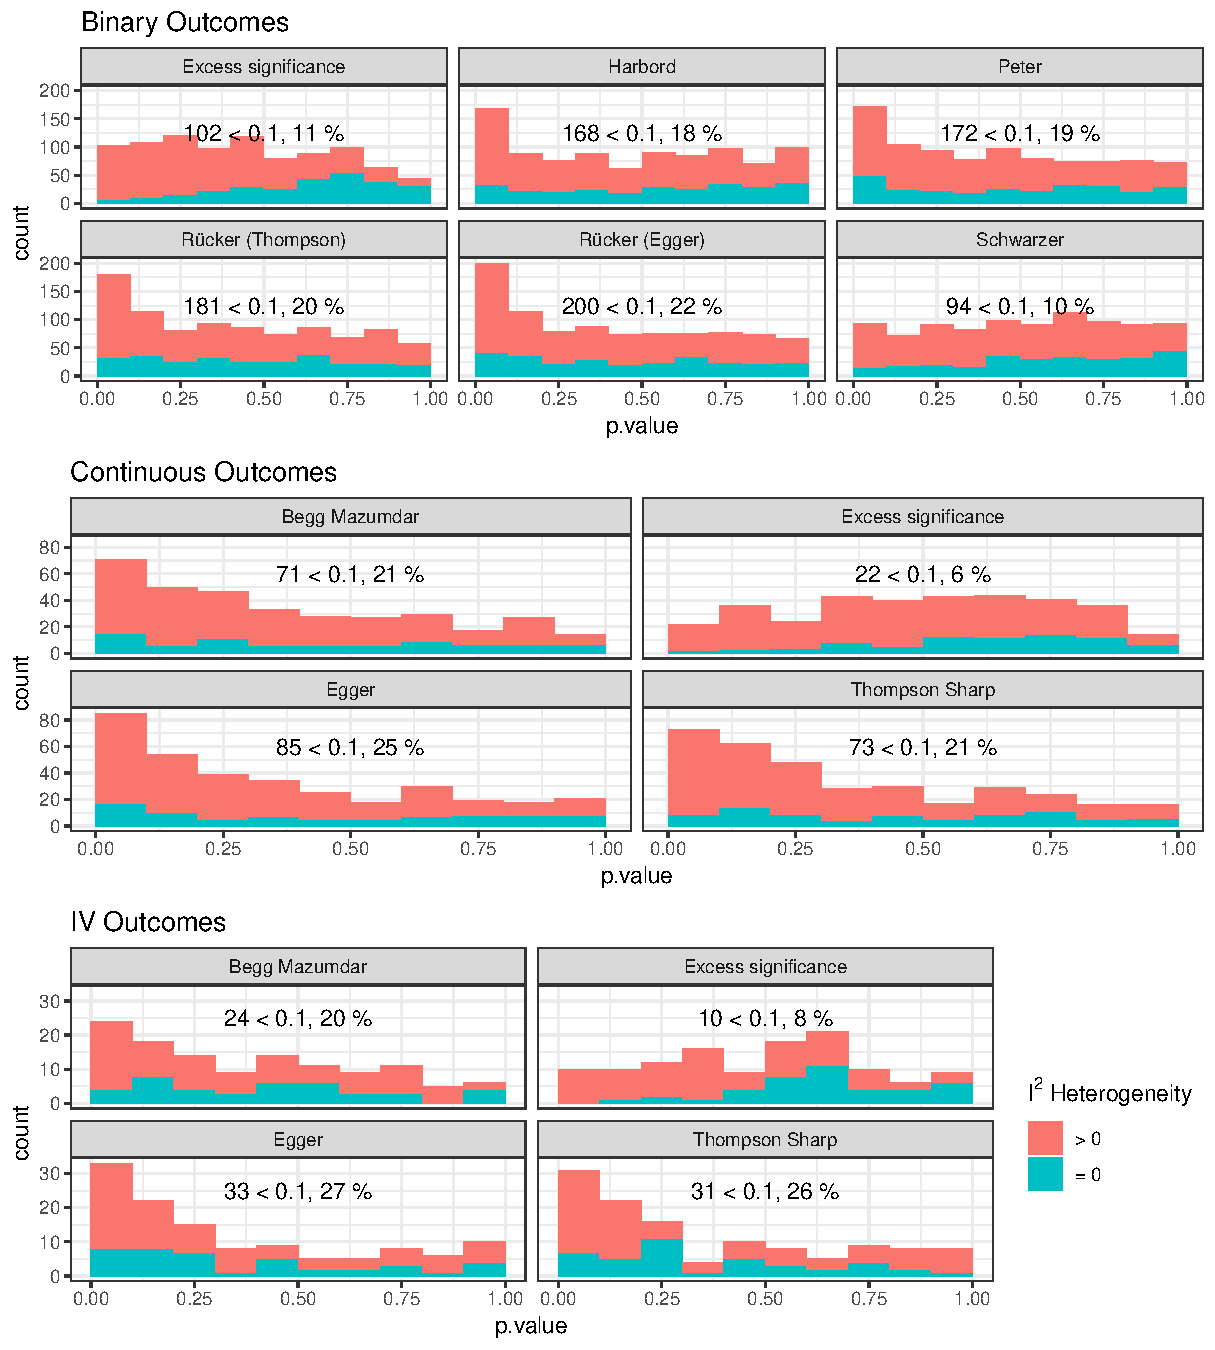
\includegraphics[width=\textwidth-3cm]{figure/ch03_figunnamed-chunk-13-1} 

}



\end{knitrout}
\caption{Mean - difference plots for publication bias adjustment methods. The mean of the adjusted treatment effects is displayed on the $x$-axis and the difference on the $y$-axis. Blue and red lines display the systematic error and the confidence intervals of the systematic error (limits of agreement). Two values have been omitted in the middle plot for Hedges $g$ and one for $z$-score (see Table \ref{missing.differences}).}
\label{fig:adjustment.mean.diff}
\end{figure}

No formal tests are provided, but the at least there seems to be no clear bias or systematic. The limits of agreement in Figure \ref{fig:adjustment.mean.diff} are large. We conclude thus that the impact of regression adjustment on the effect sizes is in general not substantially larger than the impact of Copas selection model in the subset of data where the estimate of the Copas selection model is not equal to a random effects estimate.  \\



\section{Comparison of Tests and Adjustments} \label{sec:comparison.tests.adjustment}


In section \ref{sec:change.size}, we have seen that some adjustments for small study effects are not in line with our previous definition of publication bias: Some times, the adjustment for small study effects leads to a larger treatment effect. We want to take this into account when considering evidence for publication bias. Whenever adjustment leads to larger effect sizes, the small study effect test result from section \ref{sec:publication.bias.tests} is revised and changed to negative. We will revisit the results from section \ref{sec:publication.bias.tests} and first visualize which proportion of the data finds rather ``negative publication bias'' than the predefined type of publication bias. Figure \ref{fig:test.corrected} is equal to Figure \ref{fig:test} with sole difference that now the proportion of ``negative publication bias'' is colored, and the count of significant findings is corrected (not significant for negative publication bias). \\

\begin{figure}
\begin{knitrout}
\definecolor{shadecolor}{rgb}{0.98, 0.98, 0.98}\color{fgcolor}

{\centering 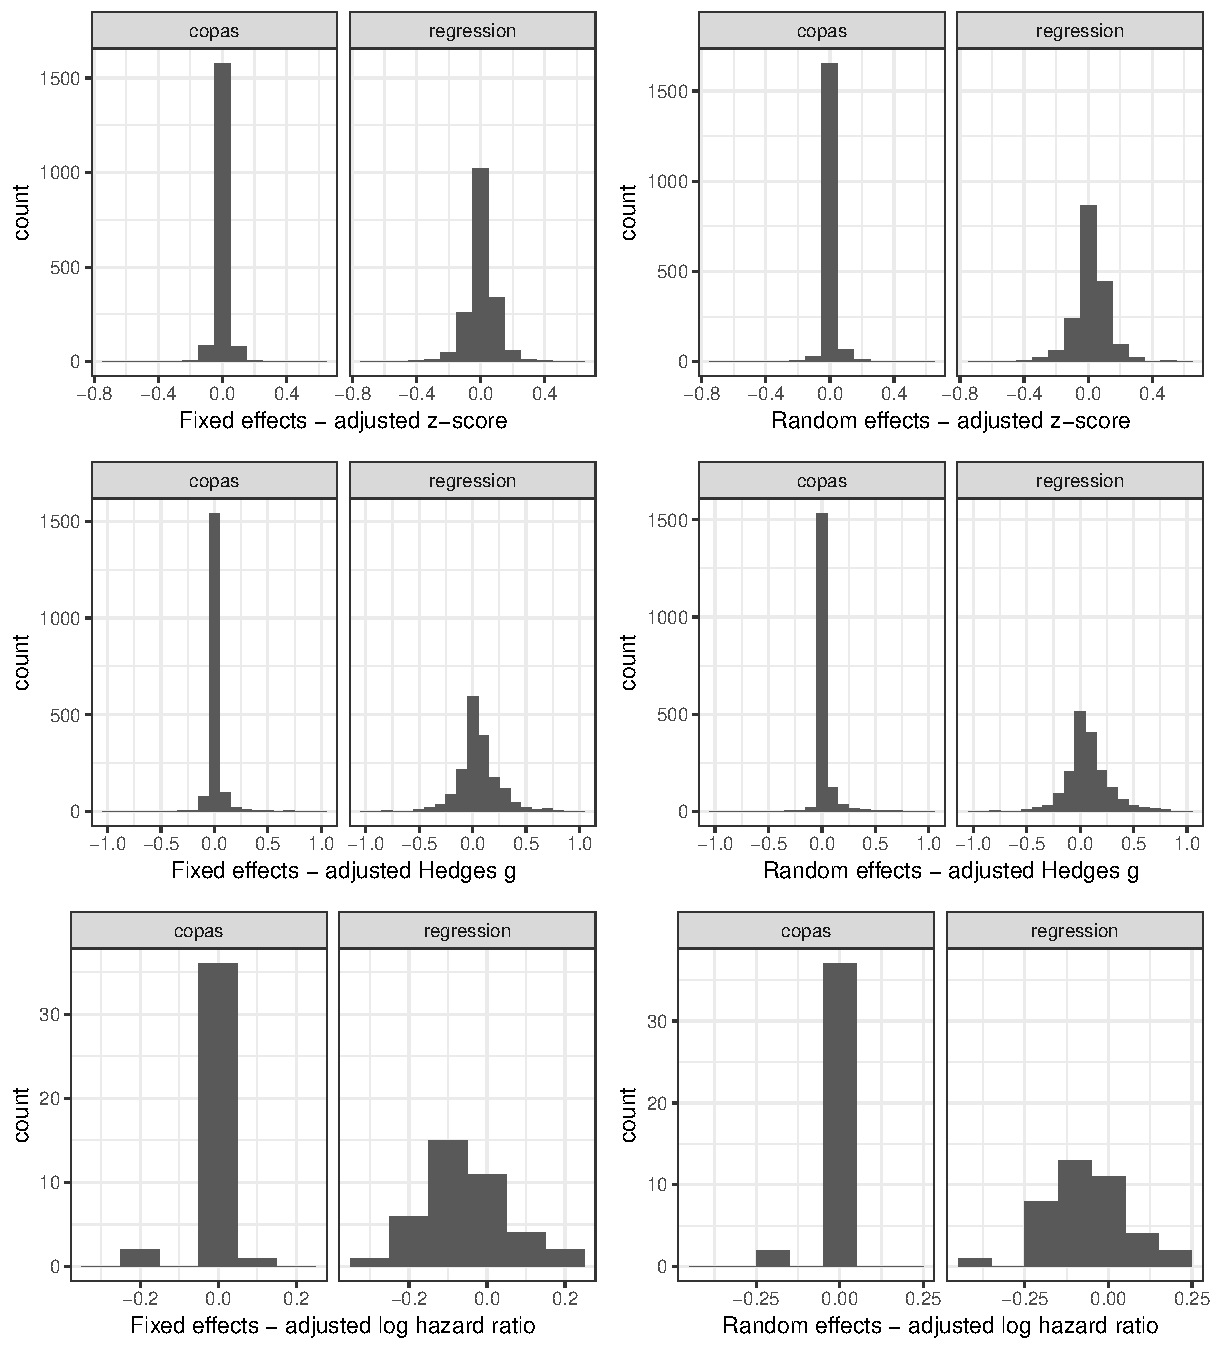
\includegraphics[width=\textwidth-3cm]{figure/ch03_figunnamed-chunk-15-1} 

}



\end{knitrout}
\caption{Histogram of the $p$-values for small study effect in meta-analyses. The testing method is indicated in the header, bin width is equal to 0.1. The significant proportion based on the threshold of 0.1 is displayed inside the figures.}
\label{fig:test.corrected}
\end{figure}

The proportion of findings where we found amplification by adjustment was 33.9\%. Most often, the proportion of tests with evidence for small study effects (and especially, excess significance), is lower, though. There are exceptions to this, such as Schwarzer's test results, where we have 143 - 60 = 83 significant test results, which corresponds to $\sim$ 40\%. Since excess significance is not necessarily connected with small study effects, we can furthermore reject the newly obtained, slightly smaller number of significant excess significance test results, and stick to the previous findings. \\
We can see how the agreement in significance is before, and after having removed negative publication bias significant results in Table \ref{test.agreement}. The proportion of agreement in significance is defined as the proportion of cases where, when the test with less significant findings is significant, also the other is significant. \\
After the adjustment of the test results, the agreement for small study effects tests and excess significance tests increases a bit. This seems also to be the general trend, but not without exceptions. The two right-most columns indicate the agreement in significance, and we see that agreement is never larger than 0.3 (with Egger's test, continuous outcomes). Furthermore, only Egger and Thompson show a goof agreement for significance ($\sim$ 0.83). In contrast, some small study effect tests for binary outcomes seem rather to be exclusive, see for example the example of Schwarzer's test (6\% after adjustment) and R\"ucker's test (11\%): Only 19 \% of the cases where Schwarzer's Test is significant have also a significant finding using R\"ucker's test. Almost all binary small study effect tests have agreement in significance > 0.5. Thus, we see that large overall agreement is rather due to the large proportion of non-significant findings.





% latex table generated in R 3.5.1 by xtable 1.8-3 package
% Mon Jul  1 14:05:18 2019
\begin{table}[ht]
\centering
\begingroup\scriptsize
\begin{tabular}{lcccc}
  & pre, overall & post, overall & pre, significance & post, significance \\ 
  \hline
\hline
Excess significance, Schwarzer & 0.81 & 0.85 & 0.12 & 0.22 \\ 
  Excess significance, Peter & 0.79 & 0.83 & 0.25 & 0.24 \\ 
  Excess significance, Rucker & 0.82 & 0.84 & 0.30 & 0.29 \\ 
  Excess significance, Harbord & 0.80 & 0.85 & 0.28 & 0.29 \\ 
  Peter, Schwarzer & 0.82 & 0.88 & 0.38 & 0.39 \\ 
  Schwarzer, Rucker & 0.82 & 0.87 & 0.32 & 0.35 \\ 
  Schwarzer, Harbord & 0.86 & 0.91 & 0.58 & 0.54 \\ 
  Rucker, Peter & 0.89 & 0.92 & 0.64 & 0.62 \\ 
  Harbord, Peter & 0.86 & 0.90 & 0.53 & 0.48 \\ 
   \hline
Excess significance, Egger & 0.80 & 0.83 & 0.67 & 0.64 \\ 
  Excess significance, Thompson & 0.81 & 0.83 & 0.55 & 0.52 \\ 
  Excess significance, Begg & 0.80 & 0.83 & 0.33 & 0.33 \\ 
  Thompson, Egger & 0.95 & 0.96 & 0.96 & 0.95 \\ 
  Thompson, Begg & 0.87 & 0.89 & 0.69 & 0.73 \\ 
  Egger, Begg & 0.86 & 0.87 & 0.78 & 0.77 \\ 
   \hline
Excess significance, Egger (survival) & 0.82 & 0.92 & 0.00 & 0.00 \\ 
  Excess significance, Thompson (survival) & 0.87 & 0.92 & 0.00 & 0.00 \\ 
  Excess significance, Begg (survival) & 0.90 & 0.95 & 0.00 & 0.00 \\ 
  Thompson, Egger (survival) & 0.90 & 0.95 & 0.67 & 0.00 \\ 
  Thompson, Begg (survival) & 0.92 & 0.97 & 0.50 & 0.00 \\ 
  Egger, Begg (survival) & 0.87 & 0.97 & 0.50 & 0.00 \\ 
   \hline
\end{tabular}
\endgroup
\caption{Overall proportion of agreement if significant or unsignificant, and for significance only. Horizontal lines separate binary, continuous and survival outcomes (order as in table). The reference significance test is the one with more significant results.} 
\label{test.agreement}
\end{table}











